%% =====================================================================
%%  CodeDuel - Final Year Project Documentation
%%  Compile with:  pdflatex main.tex  (run 2-3 times)  or  latexmk -pdf main.tex
%%  EDIT the "PROJECT DETAILS" block below with your own information.
%% =====================================================================
\documentclass[12pt,a4paper,oneside]{report}

% ---------- Packages ----------
\usepackage[utf8]{inputenc}
\usepackage[T1]{fontenc}
\usepackage[margin=1in]{geometry}
\usepackage{setspace}
\usepackage{graphicx}
\usepackage{xcolor}
\usepackage{booktabs}
\usepackage{tabularx}
\usepackage{longtable}
\usepackage{array}
\usepackage{float}
\usepackage{caption}
\usepackage{subcaption}
\usepackage{enumitem}
\usepackage{fancyhdr}
\usepackage{titlesec}
\usepackage{amsmath}
\usepackage{listings}
\usepackage{tikz}
\usetikzlibrary{shapes,arrows.meta,positioning,fit,calc,backgrounds,shadows,decorations.pathreplacing}
\usepackage{pgfplots}
\pgfplotsset{compat=1.16}
\usepackage[hidelinks,bookmarksnumbered=true]{hyperref}

% ---------- PROJECT DETAILS (edit these) ----------
\newcommand{\projecttitle}{CodeDuel: A Real-Time 1v1 Programming Battle Platform}
\newcommand{\studentname}{Your Name}
\newcommand{\rollno}{Your Roll Number}
\newcommand{\guidename}{Name of Project Guide}
\newcommand{\department}{Department of Computer Science and Engineering}
\newcommand{\university}{Name of Your University / College}
\newcommand{\academicyear}{2025--2026}
\newcommand{\degree}{Bachelor of Technology}

% ---------- Colours ----------
\definecolor{cdblue}{HTML}{1F4E79}
\definecolor{cdlight}{HTML}{DCE9F5}
\definecolor{cdgreen}{HTML}{2E7D32}
\definecolor{cdorange}{HTML}{E65100}
\definecolor{cdgrey}{HTML}{F2F2F2}
\definecolor{cdpurple}{HTML}{6A1B9A}
\definecolor{cdred}{HTML}{C62828}

% ---------- Formatting ----------
\onehalfspacing
\setlength{\parindent}{0pt}
\setlength{\parskip}{0.6em}
\titleformat{\chapter}[display]
  {\normalfont\huge\bfseries\color{cdblue}}
  {\chaptertitlename\ \thechapter}{12pt}{\Huge}
\titlespacing*{\chapter}{0pt}{-20pt}{25pt}
\titleformat{\section}{\normalfont\Large\bfseries\color{cdblue}}{\thesection}{1em}{}
\titleformat{\subsection}{\normalfont\large\bfseries}{\thesubsection}{1em}{}

\pagestyle{fancy}
\fancyhf{}
\fancyhead[L]{\small\itshape CodeDuel}
\fancyhead[R]{\small\itshape Final Year Project Report}
\fancyfoot[C]{\thepage}
\renewcommand{\headrulewidth}{0.4pt}
\fancypagestyle{plain}{\fancyhf{}\fancyfoot[C]{\thepage}\renewcommand{\headrulewidth}{0pt}}

\captionsetup{font=small,labelfont=bf}

% ---------- Code listings ----------
\lstdefinestyle{cdcode}{
  basicstyle=\ttfamily\footnotesize,
  keywordstyle=\color{cdblue}\bfseries,
  commentstyle=\color{cdgreen}\itshape,
  stringstyle=\color{cdorange},
  backgroundcolor=\color{cdgrey},
  frame=single,
  rulecolor=\color{cdblue},
  breaklines=true,
  numbers=left,
  numberstyle=\tiny\color{gray},
  captionpos=b,
  xleftmargin=1.5em,
  showstringspaces=false,
  tabsize=2
}
\lstset{style=cdcode}

% ---------- TikZ styles ----------
\tikzset{
  box/.style={rectangle,rounded corners=3pt,draw=cdblue,fill=cdlight,thick,
              minimum height=0.9cm,minimum width=2.6cm,align=center,font=\small},
  dbox/.style={cylinder,shape border rotate=90,aspect=0.25,draw=cdblue,fill=cdlight,
              thick,minimum height=1.2cm,minimum width=2.2cm,align=center,font=\small},
  state/.style={circle,draw=cdblue,fill=cdlight,thick,minimum size=1.6cm,align=center,font=\scriptsize},
  arr/.style={-{Stealth[length=2.5mm]},thick},
  darr/.style={{Stealth[length=2.5mm]}-{Stealth[length=2.5mm]},thick},
  ent/.style={rectangle,draw=cdblue,thick,fill=white,align=left,font=\scriptsize,inner sep=3pt}
}

% pie-slice helper: start angle, end angle, label, colour
\newcommand{\pieslice}[4]{%
  \pgfmathsetmacro{\midangle}{0.5*#1+0.5*#2}
  \draw[fill=#4,draw=white,thick] (0,0)--(#1:2) arc (#1:#2:2)--cycle;
  \node[font=\scriptsize,align=center] at (\midangle:3.25) {#3};}

\begin{document}

% =====================================================================
%  FRONT MATTER
% =====================================================================
\pagenumbering{roman}

% ---------- Title page ----------
\begin{titlepage}
\centering
\vspace*{0.5cm}
{\Large\bfseries\color{cdblue}\university\par}
\vspace{0.3cm}
{\large\department\par}
\vspace{1.2cm}
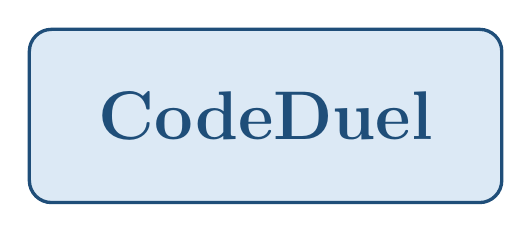
\begin{tikzpicture}
  \node[draw=cdblue,very thick,rounded corners=8pt,fill=cdlight,minimum width=6cm,minimum height=2.2cm,
        font=\Huge\bfseries\color{cdblue}] {\textbf{CodeDuel}};
\end{tikzpicture}\par
\vspace{1.2cm}
{\LARGE\bfseries \projecttitle\par}
\vspace{1.2cm}
{\large A Project Report submitted in partial fulfilment of the requirements\\
for the award of the degree of\par}
\vspace{0.4cm}
{\Large\bfseries \degree\par}
{\large in\par}
{\Large\bfseries Computer Science and Engineering\par}
\vspace{1.4cm}
\begin{tabular}{rl}
  \textbf{Submitted by:} & \studentname \\
  \textbf{Roll No.:}     & \rollno \\[1em]
  \textbf{Under the guidance of:} & \guidename \\
\end{tabular}
\vfill
{\large Academic Year \academicyear\par}
\end{titlepage}

% ---------- Certificate ----------
\chapter*{Certificate}
\addcontentsline{toc}{chapter}{Certificate}
This is to certify that the project report entitled \textbf{``\projecttitle''} submitted by
\textbf{\studentname} (Roll No.\ \rollno) in partial fulfilment of the requirements for the award of the
degree of \degree{} in Computer Science and Engineering of \university{} is a record of bona fide
work carried out by the student under my supervision and guidance during the academic year \academicyear.

The work embodied in this report has not been submitted to any other university or institute for the award
of any degree or diploma.

\vspace{3cm}
\begin{tabular}{p{7cm}p{7cm}}
\textbf{\guidename} & \textbf{Head of Department}\\
Project Guide & \department\\
\end{tabular}

% ---------- Declaration ----------
\chapter*{Declaration}
\addcontentsline{toc}{chapter}{Declaration}
I hereby declare that the project work entitled \textbf{``\projecttitle''} submitted to \university{} is a
record of original work done by me under the guidance of \textbf{\guidename}. This report has not been
submitted, in part or in full, to any other university or institution for the award of any degree, diploma
or fellowship. All sources of information used in this report have been duly acknowledged.

\vspace{2.5cm}
\begin{flushright}
\textbf{\studentname}\\ Roll No.\ \rollno\\ Date: \hspace{2cm}
\end{flushright}

% ---------- Acknowledgement ----------
\chapter*{Acknowledgement}
\addcontentsline{toc}{chapter}{Acknowledgement}
I would like to express my sincere gratitude to my project guide, \textbf{\guidename}, for the valuable
guidance, constant encouragement and constructive feedback throughout the development of this project.

I am thankful to the Head of the Department and all faculty members of the \department{} for providing the
resources and environment necessary to complete this work. I also thank my friends and family for their
support, and the open-source communities behind React, Spring Boot, PostgreSQL, Redis, Docker and Judge0,
whose tools made this project possible.

\begin{flushright}\textbf{\studentname}\end{flushright}

% ---------- Abstract ----------
\chapter*{Abstract}
\addcontentsline{toc}{chapter}{Abstract}
Competitive programming platforms are widely used for learning algorithms, yet most of them are
\emph{asynchronous}: a learner solves a problem alone and receives feedback only from an automated judge.
This removes the pressure, motivation and social element of real competition.
\textbf{CodeDuel} is a web-based, real-time platform in which two programmers are matched, receive the same
problem, write and execute code simultaneously and compete on correctness and completion time.

The system uses a \textbf{React} front end with the Monaco code editor, a \textbf{Spring Boot} back end
exposing REST APIs and WebSocket/STOMP channels, \textbf{PostgreSQL} for persistent data, \textbf{Redis} for
the matchmaking queue and temporary battle state, and a sandboxed \textbf{Judge0} service running in
\textbf{Docker} containers for safe execution of untrusted code. A rating-aware matchmaking algorithm with a
progressively widening rating window pairs players, a finite-state machine controls the life cycle of every
battle, an Elo-based rating system updates player skill after each match, and all judging and winner
decisions are made server-side to prevent client-side manipulation.

This report presents the requirement analysis, architecture, database design, algorithms, implementation,
security measures, testing and evaluation of CodeDuel, together with its limitations and future scope.

\textbf{Keywords:} Real-time systems, WebSocket, Spring Boot, React, Online judge, Matchmaking, Elo rating, Docker sandbox.

% ---------- Tables of contents ----------
\tableofcontents
\listoffigures
\listoftables

% =====================================================================
%  MAIN MATTER
% =====================================================================
\clearpage
\pagenumbering{arabic}

% ---------------------------------------------------------------------
\chapter{Introduction}
% ---------------------------------------------------------------------
\section{Background}
Programming skill is one of the most sought-after competencies in the software industry. Learners typically
practise on online judges such as LeetCode, Codeforces and HackerRank. While these platforms provide huge
problem libraries, practice is largely solitary. Live contests exist but are scheduled events with hundreds
or thousands of participants, and a beginner may feel lost in such a crowd.

A \emph{one-versus-one} format offers a middle path: short, personal, high-engagement competition available
on demand. Two players enter the same virtual room, see the same problem and race to produce a correct
solution. The opponent's progress is visible, but their source code is not, creating tension without
enabling copying.

\section{Problem Statement}
Existing practice platforms lack an on-demand, real-time, head-to-head competitive experience with fair,
secure server-side evaluation. The problem addressed by this project is:

\begin{quote}
\emph{To design and implement a scalable web platform that automatically matches two programmers, gives them
the same problem, executes their submissions securely against hidden test cases, and determines the winner
in real time while maintaining player ratings.}
\end{quote}

\section{Objectives}
\begin{itemize}[leftmargin=*]
  \item Provide secure registration, login and profile management using JWT authentication.
  \item Implement an automatic, rating-aware matchmaking system.
  \item Build a real-time battle room with a shared timer, live opponent status and instant result delivery.
  \item Execute untrusted user code safely in an isolated, resource-limited sandbox.
  \item Evaluate submissions against visible and hidden test cases and determine the winner objectively.
  \item Maintain player ratings with an Elo-style algorithm and display leaderboards and battle history.
  \item Offer Practice Mode and Private Battles for learning and easy demonstration.
\end{itemize}

\section{Scope of the Project}
\textbf{In scope:} 1v1 battles, matchmaking, private rooms, practice mode, multi-language execution
(Java, Python, C++), ratings, leaderboards, battle history and server-side judging.

\textbf{Out of scope (future work):} team battles, tournaments, video/voice chat, plagiarism detection using
machine learning, and mobile native applications.

\section{Methodology}
An \emph{incremental} development model was followed. The project was divided into four phases
(Figure~\ref{fig:phases}), where each phase yields a working, testable product. This avoids the risk of
building an over-large system that is never completed.

\begin{figure}[H]
\centering
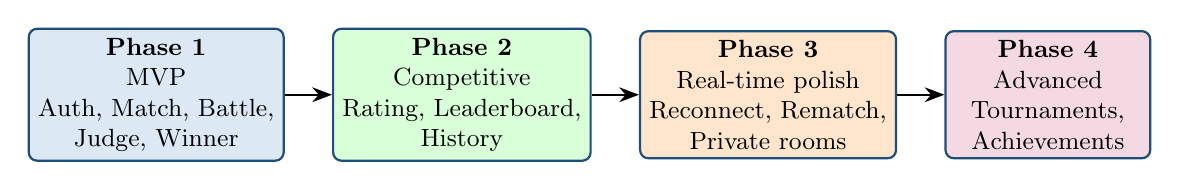
\begin{tikzpicture}[node distance=0.6cm]
  \node[box,fill=cdlight] (p1) {\textbf{Phase 1}\\MVP\\Auth, Match, Battle,\\Judge, Winner};
  \node[box,right=of p1,fill=green!15] (p2) {\textbf{Phase 2}\\Competitive\\Rating, Leaderboard,\\History};
  \node[box,right=of p2,fill=orange!20] (p3) {\textbf{Phase 3}\\Real-time polish\\Reconnect, Rematch,\\Private rooms};
  \node[box,right=of p3,fill=purple!15] (p4) {\textbf{Phase 4}\\Advanced\\Tournaments,\\Achievements};
  \draw[arr] (p1)--(p2); \draw[arr] (p2)--(p3); \draw[arr] (p3)--(p4);
\end{tikzpicture}
\caption{Incremental development phases}
\label{fig:phases}
\end{figure}

\section{Organisation of the Report}
Chapter~2 surveys related work. Chapter~3 presents requirement analysis. Chapter~4 describes the system
design. Chapter~5 details the implementation and core algorithms. Chapter~6 discusses security.
Chapter~7 covers testing, and Chapter~8 evaluates results. Chapter~9 concludes with future scope.

% ---------------------------------------------------------------------
\chapter{Literature Survey and Existing Systems}
% ---------------------------------------------------------------------
\section{Overview of Online Judge Systems}
An online judge compiles and runs submitted code against test cases and returns a verdict such as
\emph{Accepted}, \emph{Wrong Answer} or \emph{Time Limit Exceeded}. Popular systems include LeetCode,
Codeforces, HackerRank and CodeChef. Open-source judge engines such as Judge0 expose the same capability
through an API, enabling developers to embed code execution in their own products.

\section{Comparison with Existing Platforms}
\begin{table}[H]
\centering
\small
\begin{tabularx}{\textwidth}{@{}lXXXX@{}}
\toprule
\textbf{Feature} & \textbf{LeetCode} & \textbf{Codeforces} & \textbf{HackerRank} & \textbf{CodeDuel} \\
\midrule
On-demand 1v1 battles      & No  & No  & No  & \textbf{Yes} \\
Live opponent status       & No  & Scoreboard only & Scoreboard only & \textbf{Yes} \\
Rating-based matchmaking   & No  & Contest rating & No & \textbf{Yes} \\
Private battle rooms       & No  & Limited & Limited & \textbf{Yes} \\
Practice mode              & Yes & Yes & Yes & \textbf{Yes} \\
Server-side hidden tests   & Yes & Yes & Yes & \textbf{Yes} \\
Open-source / self-hostable& No  & No  & No  & \textbf{Yes} \\
\bottomrule
\end{tabularx}
\caption{Feature comparison with existing platforms}
\end{table}

\section{Related Technologies}
\begin{itemize}[leftmargin=*]
  \item \textbf{WebSocket / STOMP:} Full-duplex, low-latency communication over a single TCP connection,
        avoiding the overhead of repeated HTTP polling.
  \item \textbf{Elo rating system:} Statistical model, originally for chess, that estimates relative skill
        from match outcomes.
  \item \textbf{Container sandboxing:} Linux namespaces and cgroups isolate processes and limit CPU,
        memory and network access.
  \item \textbf{Redis:} In-memory data-structure store suited to queues, presence data and Pub/Sub.
\end{itemize}

\section{Research Gap}
Existing systems either support only asynchronous practice or large scheduled contests. There is no
lightweight, open, on-demand 1v1 platform combining matchmaking, real-time synchronisation and secure
judging, which CodeDuel aims to provide.

% ---------------------------------------------------------------------
\chapter{System Analysis and Requirements}
% ---------------------------------------------------------------------
\section{Functional Requirements}
\begin{table}[H]
\centering
\small
\begin{tabularx}{\textwidth}{@{}lX@{}}
\toprule
\textbf{ID} & \textbf{Requirement} \\
\midrule
FR1 & Users shall register, log in, log out and view/edit their profile. \\
FR2 & The system shall authenticate every request using JWT tokens. \\
FR3 & A user shall be able to join the matchmaking queue and cancel the search. \\
FR4 & The system shall match two waiting players, preferring similar ratings. \\
FR5 & Both players shall receive the same problem and a synchronised countdown/timer. \\
FR6 & Players shall write code in a browser editor and choose Java, Python or C++. \\
FR7 & Players shall be able to \emph{Run} code on sample tests and \emph{Submit} for full judging. \\
FR8 & The system shall display opponent status and test-pass count, but never opponent code. \\
FR9 & The server shall determine the winner and update ratings automatically. \\
FR10 & Users shall be able to create/join private battles using a shareable code. \\
FR11 & The system shall provide practice mode, battle history and a leaderboard. \\
\bottomrule
\end{tabularx}
\caption{Functional requirements}
\end{table}

\section{Non-Functional Requirements}
\begin{table}[H]
\centering
\small
\begin{tabularx}{\textwidth}{@{}lX@{}}
\toprule
\textbf{Attribute} & \textbf{Requirement} \\
\midrule
Performance   & Real-time events delivered in under 200~ms; submission verdict within a few seconds. \\
Security      & Passwords hashed (BCrypt); untrusted code sandboxed; hidden tests never exposed. \\
Scalability   & Stateless back end; matchmaking queue and presence stored in Redis. \\
Reliability   & Graceful handling of disconnects; battle state recoverable. \\
Usability     & Clean responsive interface usable on modern browsers. \\
Maintainability & Layered architecture (controller, service, repository) with clear separation. \\
Portability   & Entire stack deployable with Docker Compose. \\
\bottomrule
\end{tabularx}
\caption{Non-functional requirements}
\end{table}

\section{Actors and Use Cases}
Figure~\ref{fig:usecase} shows the primary actors and their interactions with the system.

\begin{figure}[H]
\centering
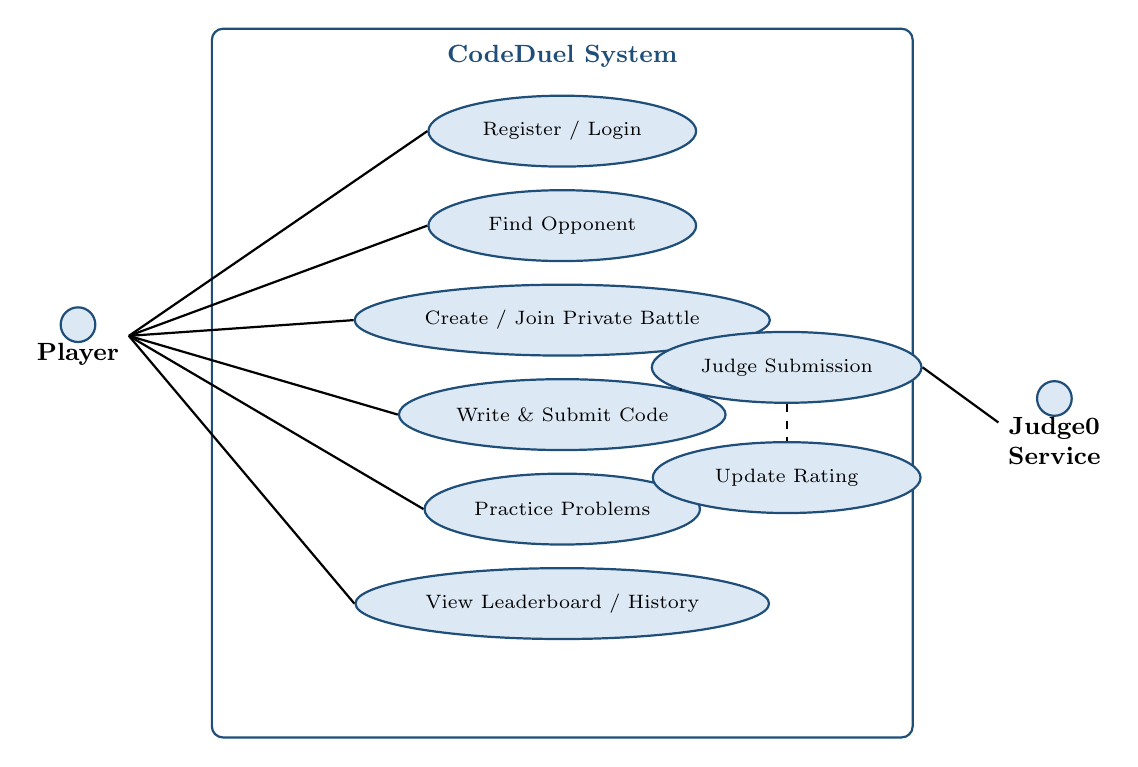
\begin{tikzpicture}[
  uc/.style={ellipse,draw=cdblue,fill=cdlight,thick,minimum width=3.4cm,minimum height=0.9cm,font=\scriptsize,align=center},
  actor/.style={draw=none,font=\small\bfseries,align=center}]
  % system boundary
  \draw[thick,cdblue,rounded corners] (-2.3,-5.6) rectangle (6.6,3.4);
  \node[font=\small\bfseries,cdblue] at (2.15,3.05) {CodeDuel System};
  % use cases
  \node[uc] (u1) at (2.15,2.1) {Register / Login};
  \node[uc] (u2) at (2.15,0.9) {Find Opponent};
  \node[uc] (u3) at (2.15,-0.3) {Create / Join Private Battle};
  \node[uc] (u4) at (2.15,-1.5) {Write \& Submit Code};
  \node[uc] (u5) at (2.15,-2.7) {Practice Problems};
  \node[uc] (u6) at (2.15,-3.9) {View Leaderboard / History};
  \node[uc] (u7) at (5.0,-0.9) {Judge Submission};
  \node[uc] (u8) at (5.0,-2.3) {Update Rating};
  % actors
  \node[actor] (pl) at (-4,-0.5) {\tikz[baseline=-0.5ex]{\draw[thick,cdblue,fill=cdlight] (0,0) circle (0.22);}\\Player};
  \node[actor] (jd) at (8.4,-1.6) {\tikz[baseline=-0.5ex]{\draw[thick,cdblue,fill=cdlight] (0,0) circle (0.22);}\\Judge0\\Service};
  \foreach \i in {u1,u2,u3,u4,u5,u6} \draw[thick] (pl.east) -- (\i.west);
  \draw[thick,dashed] (u4) -- (u7);
  \draw[thick,dashed] (u7) -- (u8);
  \draw[thick] (u7.east) -- (jd.west);
\end{tikzpicture}
\caption{Use case diagram of CodeDuel}
\label{fig:usecase}
\end{figure}

\section{Feasibility Study}
\textbf{Technical feasibility:} All technologies are mature, open source and well documented.
\textbf{Economic feasibility:} Free tiers of hosting, Docker and open-source software keep cost minimal.
\textbf{Operational feasibility:} The interface follows familiar coding-platform conventions, requiring
no special training.

\section{Technology Stack}
\begin{table}[H]
\centering
\small
\begin{tabularx}{\textwidth}{@{}llX@{}}
\toprule
\textbf{Layer} & \textbf{Technology} & \textbf{Purpose} \\
\midrule
Front end       & React, Tailwind CSS & Component-based responsive UI \\
Code editor     & Monaco Editor       & VS Code editing experience in browser \\
Back end        & Spring Boot (Java)  & REST APIs, business logic \\
Real-time       & WebSocket + STOMP   & Bidirectional battle events \\
Security        & Spring Security, JWT& Authentication and authorisation \\
Database        & PostgreSQL, JPA     & Persistent relational data \\
Cache / queue   & Redis               & Matchmaking queue, presence, battle state \\
Code execution  & Judge0              & Sandboxed compilation and execution \\
Container       & Docker, Compose     & Isolation and deployment \\
Tools           & Maven, Git, Postman, Swagger & Build, VCS, API testing, documentation \\
\bottomrule
\end{tabularx}
\caption{Technology stack}
\end{table}

% ---------------------------------------------------------------------
\chapter{System Design}
% ---------------------------------------------------------------------
\section{Overall Architecture}
CodeDuel follows a client--server architecture with a layered Spring Boot back end. The React client uses
REST for request/response operations and WebSocket for real-time events. User code is never executed in the
application server; it is forwarded to the isolated Judge0 service.

\begin{figure}[H]
\centering
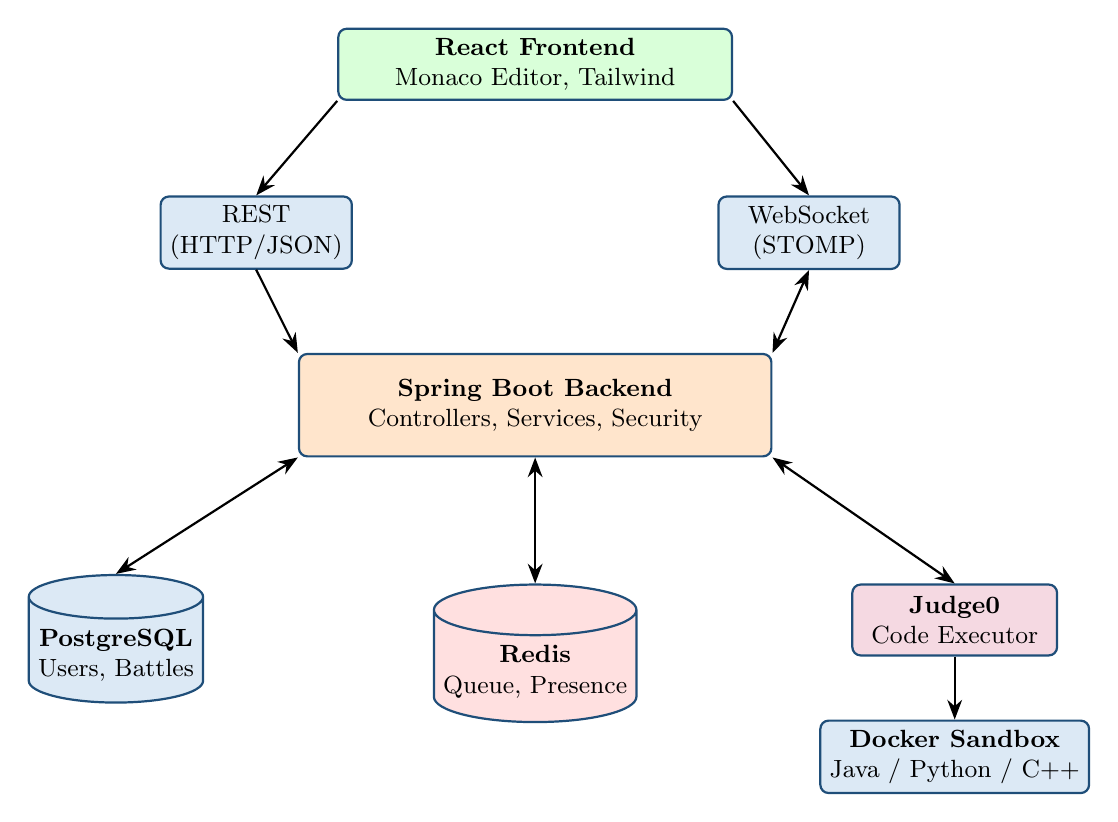
\begin{tikzpicture}[node distance=1.1cm and 1.6cm]
  \node[box,minimum width=5cm,fill=green!15] (react) {\textbf{React Frontend}\\Monaco Editor, Tailwind};
  \node[box,below left=1.2cm and -0.2cm of react,minimum width=2.3cm] (rest) {REST\\(HTTP/JSON)};
  \node[box,below right=1.2cm and -0.2cm of react,minimum width=2.3cm] (ws) {WebSocket\\(STOMP)};
  \node[box,below=3.2cm of react,minimum width=6cm,minimum height=1.3cm,fill=orange!20] (spring)
        {\textbf{Spring Boot Backend}\\Controllers, Services, Security};
  \node[dbox,below left=1.6cm and 1.4cm of spring] (pg) {\textbf{PostgreSQL}\\Users, Battles};
  \node[dbox,below=1.6cm of spring,fill=red!12] (redis) {\textbf{Redis}\\Queue, Presence};
  \node[box,below right=1.6cm and 1.0cm of spring,fill=purple!15] (judge) {\textbf{Judge0}\\Code Executor};
  \node[box,below=0.8cm of judge,fill=cdlight] (docker) {\textbf{Docker Sandbox}\\Java / Python / C++};
  \draw[arr] (react.south west)--(rest.north);
  \draw[arr] (react.south east)--(ws.north);
  \draw[arr] (rest.south)--(spring.north west);
  \draw[darr] (ws.south)--(spring.north east);
  \draw[darr] (spring.south west)--(pg.north);
  \draw[darr] (spring)--(redis);
  \draw[darr] (spring.south east)--(judge.north);
  \draw[arr] (judge)--(docker);
\end{tikzpicture}
\caption{High-level system architecture}
\label{fig:arch}
\end{figure}

\section{Backend Layered Architecture}
\begin{figure}[H]
\centering
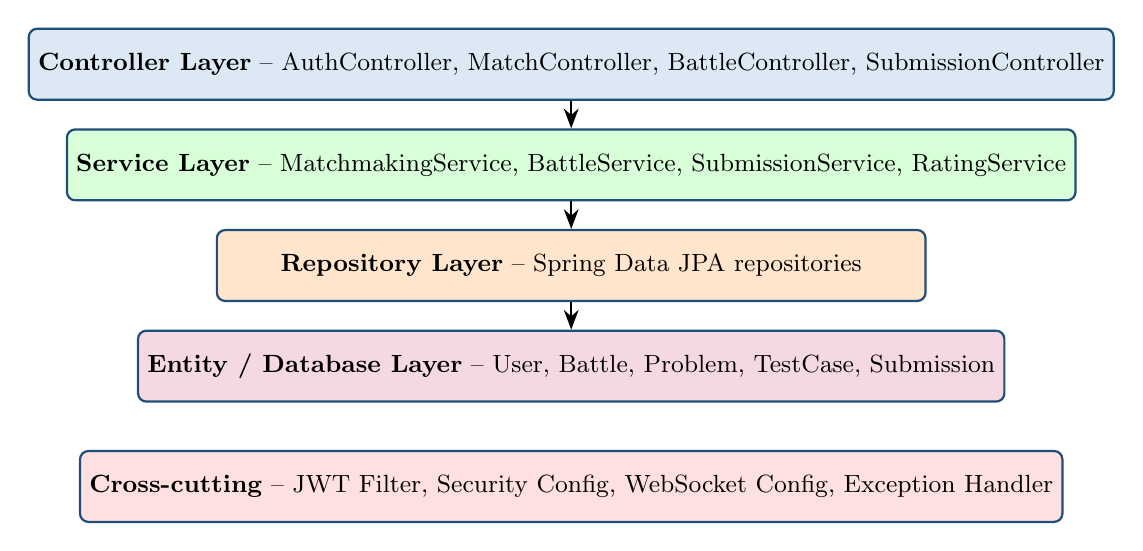
\begin{tikzpicture}[node distance=0.35cm]
  \node[box,minimum width=9cm,fill=cdlight] (c) {\textbf{Controller Layer} -- AuthController, MatchController, BattleController, SubmissionController};
  \node[box,minimum width=9cm,below=of c,fill=green!15] (s) {\textbf{Service Layer} -- MatchmakingService, BattleService, SubmissionService, RatingService};
  \node[box,minimum width=9cm,below=of s,fill=orange!20] (r) {\textbf{Repository Layer} -- Spring Data JPA repositories};
  \node[box,minimum width=9cm,below=of r,fill=purple!15] (e) {\textbf{Entity / Database Layer} -- User, Battle, Problem, TestCase, Submission};
  \draw[arr] (c)--(s); \draw[arr] (s)--(r); \draw[arr] (r)--(e);
  \node[box,minimum width=9cm,below=0.6cm of e,fill=red!12] {\textbf{Cross-cutting} -- JWT Filter, Security Config, WebSocket Config, Exception Handler};
\end{tikzpicture}
\caption{Layered structure of the Spring Boot backend}
\end{figure}

\section{Battle Life Cycle (State Machine)}
Each battle is modelled as a finite-state machine. State transitions occur only on the server, guaranteeing
consistency between both players.

\begin{figure}[H]
\centering
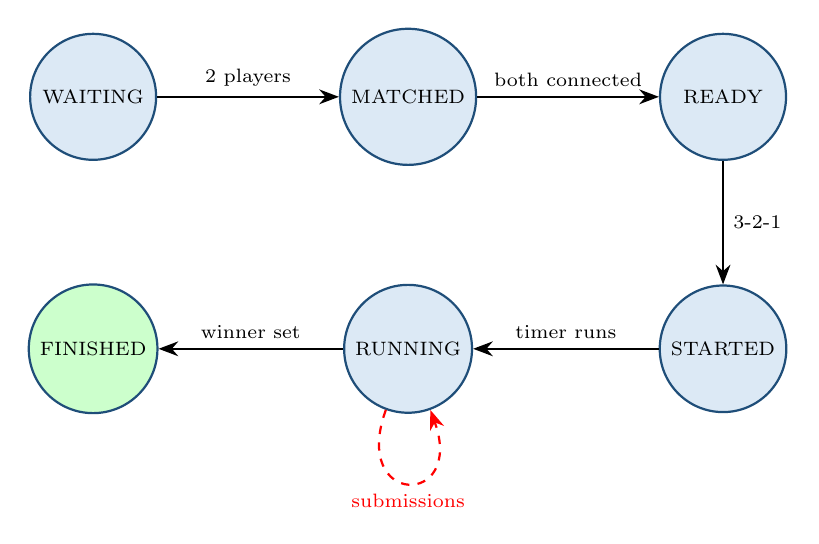
\begin{tikzpicture}
  \node[state] (w) at (0,0) {WAITING};
  \node[state] (m) at (4,0) {MATCHED};
  \node[state] (r) at (8,0) {READY};
  \node[state] (s) at (8,-3.2) {STARTED};
  \node[state] (u) at (4,-3.2) {RUNNING};
  \node[state,fill=green!20] (f) at (0,-3.2) {FINISHED};
  \draw[arr] (w)--(m) node[midway,above,font=\scriptsize]{2 players};
  \draw[arr] (m)--(r) node[midway,above,font=\scriptsize]{both connected};
  \draw[arr] (r)--(s) node[midway,right,font=\scriptsize]{3-2-1};
  \draw[arr] (s)--(u) node[midway,above,font=\scriptsize]{timer runs};
  \draw[arr] (u)--(f) node[midway,above,font=\scriptsize]{winner set};
  \draw[arr,dashed,red] (u) to[out=250,in=290,looseness=6] node[font=\scriptsize,below,pos=0.5]{submissions} (u);
\end{tikzpicture}
\caption{Battle state machine}
\label{fig:state}
\end{figure}

\begin{table}[H]
\centering
\small
\begin{tabularx}{\textwidth}{@{}lXl@{}}
\toprule
\textbf{State} & \textbf{Meaning} & \textbf{Trigger} \\
\midrule
WAITING  & Player is in queue or private room is open & Find Opponent / Create room \\
MATCHED  & Two players paired, battle record created  & Matchmaker \\
READY    & Both WebSocket connections established    & Client join events \\
STARTED  & Countdown finished; problem revealed       & Server timer \\
RUNNING  & Players coding and submitting              & Submissions \\
FINISHED & Winner decided, ratings updated            & All accepted / time up \\
\bottomrule
\end{tabularx}
\caption{Battle states}
\end{table}

\section{Matchmaking Flow}
\begin{figure}[H]
\centering
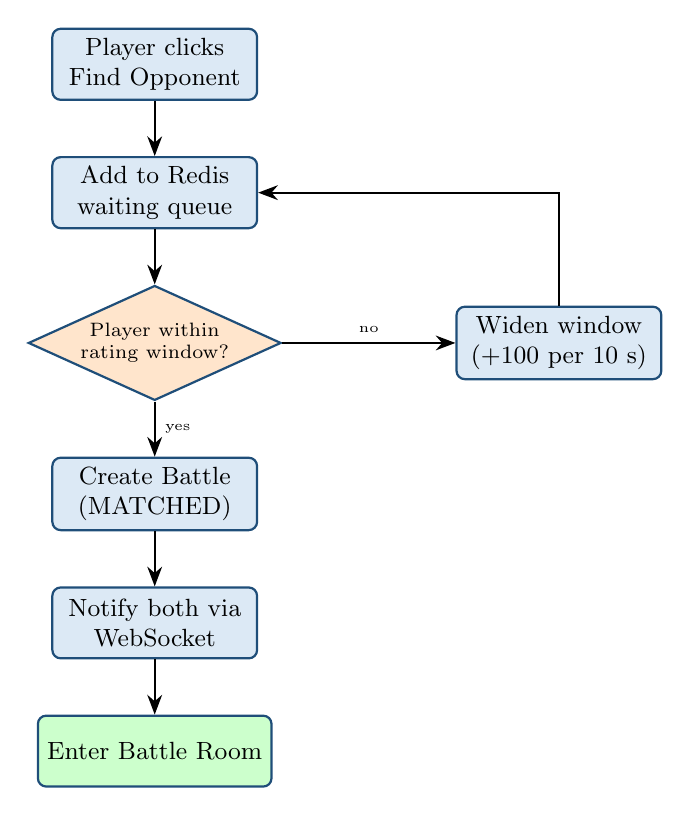
\begin{tikzpicture}[node distance=0.7cm,
  dec/.style={diamond,draw=cdblue,fill=orange!20,thick,aspect=2.2,font=\scriptsize,align=center,inner sep=1pt}]
  \node[box] (a) {Player clicks\\Find Opponent};
  \node[box,below=of a] (b) {Add to Redis\\waiting queue};
  \node[dec,below=of b] (c) {Player within\\rating window?};
  \node[box,right=2.2cm of c] (d) {Widen window\\(+100 per 10 s)};
  \node[box,below=of c] (e) {Create Battle\\(MATCHED)};
  \node[box,below=of e] (f) {Notify both via\\WebSocket};
  \node[box,below=of f,fill=green!20] (g) {Enter Battle Room};
  \draw[arr] (a)--(b); \draw[arr] (b)--(c);
  \draw[arr] (c)--(e) node[midway,right,font=\tiny]{yes};
  \draw[arr] (c)--(d) node[midway,above,font=\tiny]{no};
  \draw[arr] (d) |- (b);
  \draw[arr] (e)--(f); \draw[arr] (f)--(g);
\end{tikzpicture}
\caption{Matchmaking flowchart}
\end{figure}

\section{Sequence Diagram: Submission and Judging}
\begin{figure}[H]
\centering
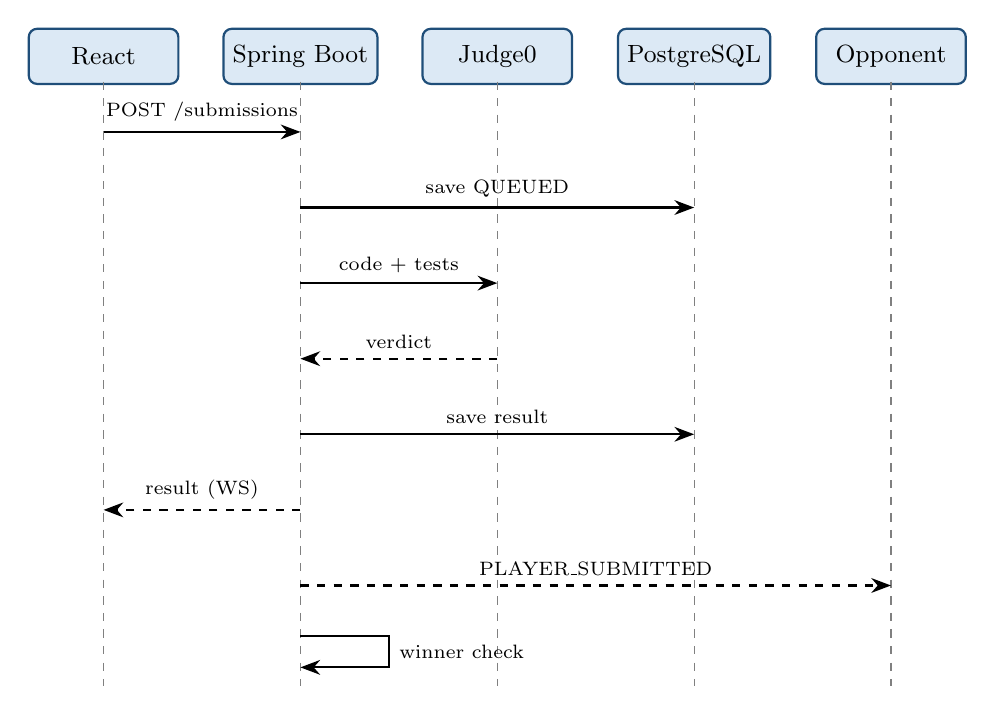
\begin{tikzpicture}[x=2.5cm,y=0.8cm,font=\scriptsize]
  \foreach \x/\n in {0/React,1/Spring Boot,2/Judge0,3/PostgreSQL,4/Opponent} {
    \node[box,minimum width=1.9cm,minimum height=0.7cm] (n\x) at (\x,0) {\n};
    \draw[dashed,gray] (\x,-0.4)--(\x,-10);
  }
  \draw[arr] (0,-1.2)--(1,-1.2) node[midway,above]{POST /submissions};
  \draw[arr] (1,-2.4)--(3,-2.4) node[midway,above]{save QUEUED};
  \draw[arr] (1,-3.6)--(2,-3.6) node[midway,above]{code + tests};
  \draw[arr,dashed] (2,-4.8)--(1,-4.8) node[midway,above]{verdict};
  \draw[arr] (1,-6.0)--(3,-6.0) node[midway,above]{save result};
  \draw[arr,dashed] (1,-7.2)--(0,-7.2) node[midway,above]{result (WS)};
  \draw[arr,dashed] (1,-8.4)--(4,-8.4) node[midway,above]{PLAYER\_SUBMITTED};
  \draw[arr] (1,-9.2)--(1.45,-9.2) |- (1,-9.7) node[pos=0.25,right]{winner check};
\end{tikzpicture}
\caption{Sequence of a code submission}
\end{figure}

\section{Database Design}
\subsection{Entity--Relationship Diagram}
\begin{figure}[H]
\centering
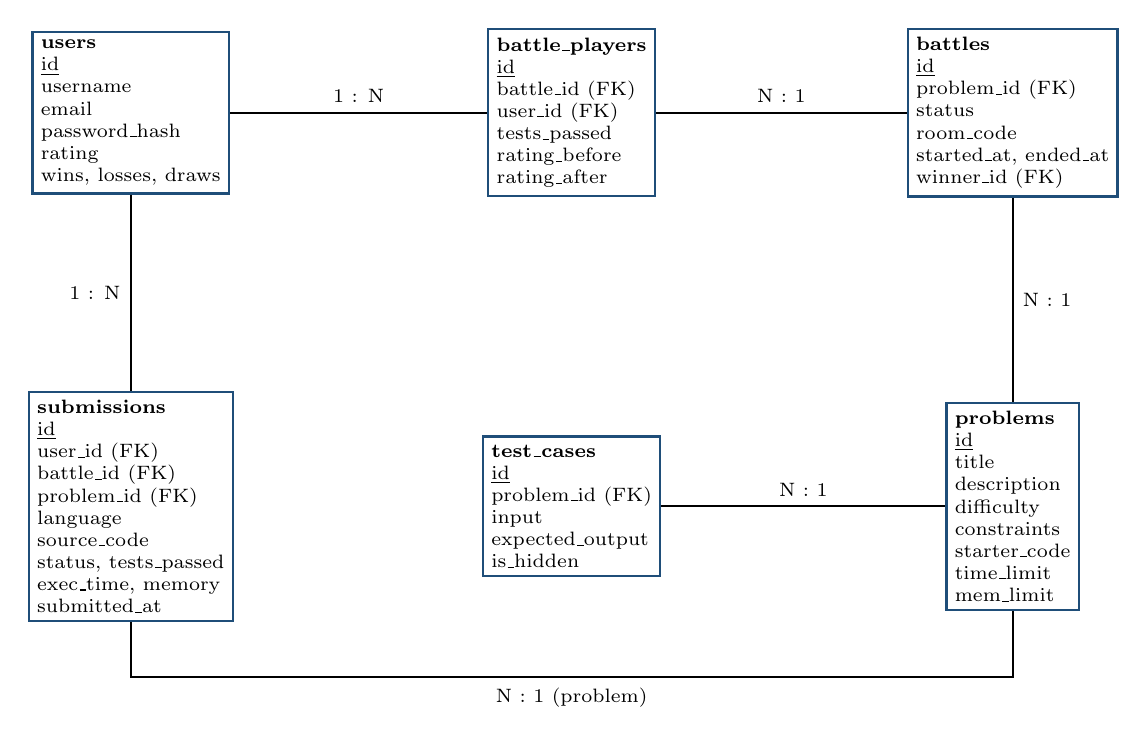
\begin{tikzpicture}
  \node[ent] (user) at (0,0) {\textbf{users}\\\underline{id}\\username\\email\\password\_hash\\rating\\wins, losses, draws};
  \node[ent] (bp) at (5.6,0) {\textbf{battle\_players}\\\underline{id}\\battle\_id (FK)\\user\_id (FK)\\tests\_passed\\rating\_before\\rating\_after};
  \node[ent] (battle) at (11.2,0) {\textbf{battles}\\\underline{id}\\problem\_id (FK)\\status\\room\_code\\started\_at, ended\_at\\winner\_id (FK)};
  \node[ent] (sub) at (0,-5) {\textbf{submissions}\\\underline{id}\\user\_id (FK)\\battle\_id (FK)\\problem\_id (FK)\\language\\source\_code\\status, tests\_passed\\exec\_time, memory\\submitted\_at};
  \node[ent] (tc) at (5.6,-5) {\textbf{test\_cases}\\\underline{id}\\problem\_id (FK)\\input\\expected\_output\\is\_hidden};
  \node[ent] (prob) at (11.2,-5) {\textbf{problems}\\\underline{id}\\title\\description\\difficulty\\constraints\\starter\_code\\time\_limit\\mem\_limit};
  \draw[thick] (user)--(bp) node[midway,above,font=\scriptsize]{1 : N};
  \draw[thick] (bp)--(battle) node[midway,above,font=\scriptsize]{N : 1};
  \draw[thick] (user)--(sub) node[midway,left,font=\scriptsize]{1 : N};
  \draw[thick] (battle)--(prob) node[midway,right,font=\scriptsize]{N : 1};
  \draw[thick] (tc)--(prob) node[midway,above,font=\scriptsize]{N : 1};
  \draw[thick] (sub.south) -- ++(0,-0.7) -| (prob.south) node[pos=0.25,below,font=\scriptsize]{N : 1 (problem)};
\end{tikzpicture}
\caption{Entity--relationship diagram}
\label{fig:er}
\end{figure}

\subsection{Table Descriptions}
\begin{table}[H]
\centering
\small
\begin{tabularx}{\textwidth}{@{}lX@{}}
\toprule
\textbf{Table} & \textbf{Description} \\
\midrule
users          & Account credentials, current rating and win/loss/draw statistics. \\
problems       & Problem statements, difficulty, constraints, starter code and limits. \\
test\_cases    & Visible and hidden input/expected-output pairs for each problem. \\
battles        & One row per match: status, problem, timing and winner. \\
battle\_players& Join table linking two users to a battle with per-player results and rating change. \\
submissions    & Every run/submit with language, verdict, tests passed, time and memory. \\
\bottomrule
\end{tabularx}
\caption{Database tables}
\end{table}

\subsection{Use of Redis}
\begin{table}[H]
\centering
\small
\begin{tabularx}{\textwidth}{@{}llX@{}}
\toprule
\textbf{Key pattern} & \textbf{Type} & \textbf{Purpose} \\
\midrule
\texttt{waiting\_players}   & Sorted set (score = rating) & Matchmaking queue \\
\texttt{battle:\{id\}}      & Hash   & Temporary live battle state \\
\texttt{player:\{id\}}      & String (TTL) & Online / presence status \\
\texttt{battle:events}      & Pub/Sub channel & Cross-instance event broadcast \\
\bottomrule
\end{tabularx}
\caption{Redis data usage}
\end{table}

\section{API Design}
\subsection{REST Endpoints}
\begin{table}[H]
\centering
\small
\begin{tabularx}{\textwidth}{@{}llX@{}}
\toprule
\textbf{Method} & \textbf{Endpoint} & \textbf{Description} \\
\midrule
POST & \texttt{/api/auth/register} & Create a new user account \\
POST & \texttt{/api/auth/login}    & Authenticate and return JWT \\
GET  & \texttt{/api/profile}       & Current user's profile and statistics \\
GET  & \texttt{/api/problems/\{id\}} & Fetch problem (visible tests only) \\
POST & \texttt{/api/matchmaking/join}  & Join matchmaking queue \\
POST & \texttt{/api/battles/private}   & Create private battle, returns code \\
POST & \texttt{/api/submissions}   & Submit code for judging \\
GET  & \texttt{/api/leaderboard}   & Top players by rating \\
GET  & \texttt{/api/battles/history} & Past battles of the user \\
\bottomrule
\end{tabularx}
\caption{Main REST API endpoints}
\end{table}

\subsection{WebSocket Events}
\begin{table}[H]
\centering
\small
\begin{tabularx}{\textwidth}{@{}llX@{}}
\toprule
\textbf{Event} & \textbf{Direction} & \textbf{Description} \\
\midrule
PLAYER\_JOINED       & Server $\to$ Clients & Opponent entered the room \\
BATTLE\_STARTED      & Server $\to$ Clients & Countdown ended, problem shown \\
PLAYER\_SUBMITTED    & Server $\to$ Opponent & Opponent submitted; tests passed count \\
PLAYER\_DISCONNECTED & Server $\to$ Opponent & Opponent lost connection \\
TIMER\_SYNC          & Server $\to$ Clients & Authoritative remaining time \\
BATTLE\_FINISHED     & Server $\to$ Clients & Winner, scores, rating changes \\
\bottomrule
\end{tabularx}
\caption{WebSocket events on channel \texttt{/topic/battle/\{battleId\}}}
\end{table}

\section{User Interface Design}
Figure~\ref{fig:battleui} shows the wire-frame of the battle room, the core screen of the application.

\begin{figure}[H]
\centering
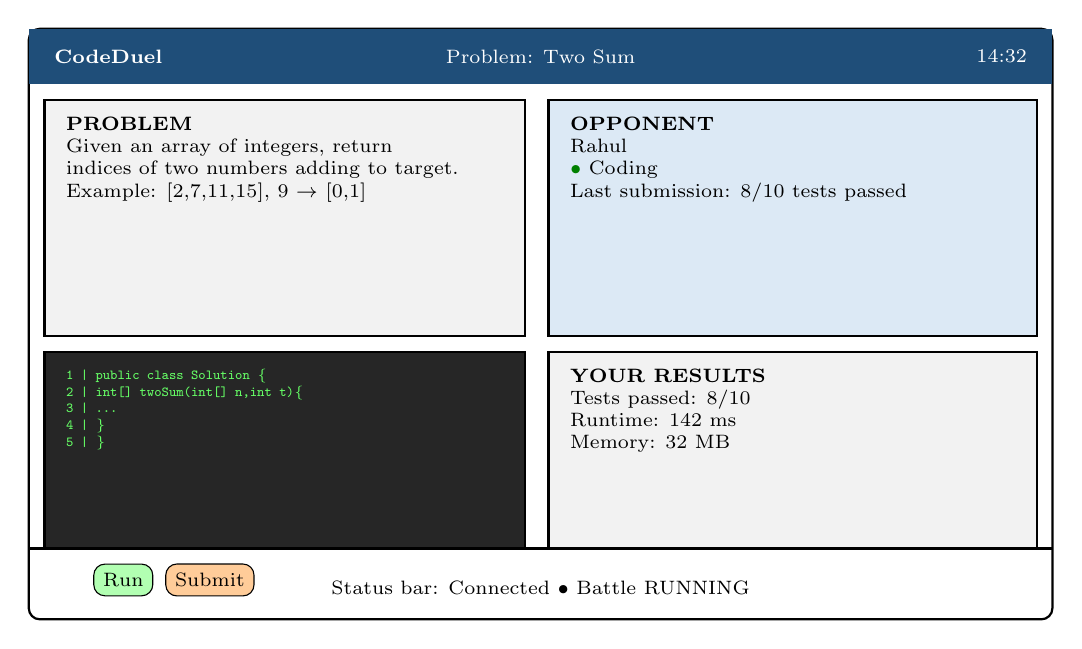
\begin{tikzpicture}[font=\scriptsize]
  \draw[thick,rounded corners,fill=white] (0,0) rectangle (13,7.5);
  \fill[cdblue] (0,6.8) rectangle (13,7.5);
  \node[white,anchor=west] at (0.2,7.15) {\textbf{CodeDuel}};
  \node[white] at (6.5,7.15) {Problem: Two Sum};
  \node[white,anchor=east] at (12.8,7.15) {14:32};
  % problem panel
  \draw[thick,fill=cdgrey] (0.2,3.6) rectangle (6.3,6.6);
  \node[anchor=north west,align=left] at (0.35,6.5) {\textbf{PROBLEM}\\Given an array of integers, return\\indices of two numbers adding to target.\\Example: [2,7,11,15], 9 $\to$ [0,1]};
  % editor
  \draw[thick,fill=black!85] (0.2,0.9) rectangle (6.3,3.4);
  \node[anchor=north west,text=green!60,align=left,font=\ttfamily\tiny] at (0.35,3.3) {1 | public class Solution \{\\2 |   int[] twoSum(int[] n,int t)\{\\3 |     ...\\4 |   \}\\5 | \}};
  \node[draw,fill=green!30,rounded corners] at (1.2,0.5) {Run};
  \node[draw,fill=orange!40,rounded corners] at (2.3,0.5) {Submit};
  % opponent
  \draw[thick,fill=cdlight] (6.6,3.6) rectangle (12.8,6.6);
  \node[anchor=north west,align=left] at (6.75,6.5) {\textbf{OPPONENT}\\Rahul\\{\color{green!50!black}$\bullet$} Coding\\Last submission: 8/10 tests passed};
  \draw[thick,fill=cdgrey] (6.6,0.9) rectangle (12.8,3.4);
  \node[anchor=north west,align=left] at (6.75,3.3) {\textbf{YOUR RESULTS}\\Tests passed: 8/10\\Runtime: 142 ms\\Memory: 32 MB};
  \draw[thick] (0,0.9)--(13,0.9);
  \node at (6.5,0.4) {Status bar: Connected $\bullet$ Battle RUNNING};
\end{tikzpicture}
\caption{Wire-frame of the Battle Room}
\label{fig:battleui}
\end{figure}

% ---------------------------------------------------------------------
\chapter{Implementation}
% ---------------------------------------------------------------------
\section{Project Structure}
\begin{lstlisting}[language=,caption={Backend and frontend structure},numbers=none]
codeduel/
|-- backend/ (Spring Boot)
|   |-- controller/  AuthController, MatchController, BattleController ...
|   |-- service/     MatchmakingService, BattleService, RatingService ...
|   |-- repository/  UserRepository, BattleRepository, ...
|   |-- entity/      User, Battle, Problem, TestCase, Submission
|   |-- websocket/   WebSocketConfig, BattleWebSocketController
|   `-- security/    JwtAuthenticationFilter, SecurityConfig
`-- frontend/ (React)
    |-- components/  CodeEditor, ProblemPanel, Timer, PlayerCard ...
    |-- pages/       Login, Home, Matchmaking, Battle, Results, Profile
    |-- services/    api.js, auth.js, websocket.js
    `-- context/     AuthContext
\end{lstlisting}

\section{Authentication with JWT}
Passwords are hashed using BCrypt. On login the server issues a signed JSON Web Token, which the client sends
in the \texttt{Authorization: Bearer} header. A filter validates the token on every request and also secures
the WebSocket handshake.

\begin{lstlisting}[language=Java,caption={Simplified JWT authentication filter}]
public class JwtAuthenticationFilter extends OncePerRequestFilter {
  @Override
  protected void doFilterInternal(HttpServletRequest req,
        HttpServletResponse res, FilterChain chain)
        throws ServletException, IOException {
    String header = req.getHeader("Authorization");
    if (header != null && header.startsWith("Bearer ")) {
      String token = header.substring(7);
      if (jwtService.isValid(token)) {
        String username = jwtService.extractUsername(token);
        UserDetails user = userDetailsService.loadUserByUsername(username);
        var auth = new UsernamePasswordAuthenticationToken(
                user, null, user.getAuthorities());
        SecurityContextHolder.getContext().setAuthentication(auth);
      }
    }
    chain.doFilter(req, res);
  }
}
\end{lstlisting}

\section{Matchmaking Algorithm}
Players wait in a Redis sorted set keyed by rating. A scheduled task runs every second. For each waiting
player the acceptable rating difference grows with waiting time:
\[
  \Delta_{\max}(t) = 100 \times \left(\left\lfloor \frac{t}{10} \right\rfloor + 1\right),
\]
where $t$ is the waiting time in seconds. A pair is created when
$|R_A - R_B| \le \min(\Delta_{\max}(t_A),\,\Delta_{\max}(t_B))$ or, to reduce waiting, the maximum of both.

\begin{table}[H]
\centering
\small
\begin{tabular}{@{}cc@{}}
\toprule
\textbf{Waiting time (s)} & \textbf{Allowed rating difference} \\
\midrule
0--10  & $\pm 100$ \\
10--20 & $\pm 200$ \\
20--30 & $\pm 300$ \\
$>30$  & $\pm 400$ or any available player \\
\bottomrule
\end{tabular}
\caption{Expanding rating window}
\end{table}

\begin{lstlisting}[language=Java,caption={Matchmaking scheduler (simplified)}]
@Scheduled(fixedDelay = 1000)
public void matchPlayers() {
  Set<ZSetOperations.TypedTuple<String>> players =
      redis.opsForZSet().rangeWithScores("waiting_players", 0, -1);
  List<Candidate> list = toCandidates(players);   // id, rating, joinedAt
  for (Candidate a : list) {
    int window = 100 * ((int)(a.waitSeconds() / 10) + 1);
    for (Candidate b : list) {
      if (a.id().equals(b.id())) continue;
      if (Math.abs(a.rating() - b.rating()) <= window) {
        redis.opsForZSet().remove("waiting_players", a.id(), b.id());
        battleService.createBattle(a.id(), b.id());
        return;
      }
    }
  }
}
\end{lstlisting}

\section{WebSocket Configuration}
\begin{lstlisting}[language=Java,caption={STOMP over WebSocket configuration}]
@Configuration
@EnableWebSocketMessageBroker
public class WebSocketConfig implements WebSocketMessageBrokerConfigurer {
  @Override
  public void registerStompEndpoints(StompEndpointRegistry registry) {
    registry.addEndpoint("/ws")
            .setAllowedOriginPatterns("*").withSockJS();
  }
  @Override
  public void configureMessageBroker(MessageBrokerRegistry registry) {
    registry.enableSimpleBroker("/topic");
    registry.setApplicationDestinationPrefixes("/app");
  }
}
\end{lstlisting}

\section{Code Execution via Judge0}
When a player submits, the server creates one Judge0 request per test case (or a batch) containing the source
code, language id, stdin and expected output, along with CPU-time and memory limits. Results are collected,
counted and stored. Untrusted code never runs on the application server.

\begin{lstlisting}[language=Java,caption={Submission judging (simplified)}]
public SubmissionResult judge(Submission s, List<TestCase> tests) {
  int passed = 0;
  for (TestCase t : tests) {
    JudgeResponse r = judge0Client.execute(
        s.getSourceCode(), s.getLanguageId(),
        t.getInput(), t.getExpectedOutput(),
        problem.getTimeLimit(), problem.getMemoryLimit());
    if (r.getStatus() == Status.ACCEPTED) passed++;
    else if (r.isCompileError()) return SubmissionResult.compileError(r);
  }
  s.setTestsPassed(passed);
  s.setStatus(passed == tests.size() ? ACCEPTED : WRONG_ANSWER);
  return repository.save(s);
}
\end{lstlisting}

\section{Winner Determination}
The winner is not simply the first to submit. The decision uses a lexicographic comparison:
\begin{enumerate}[leftmargin=*]
  \item Higher number of test cases passed.
  \item If equal, earlier time of the best submission.
  \item (Optional extension) If still equal, lower execution time.
  \item If all are equal, the result is a draw.
\end{enumerate}

\begin{figure}[H]
\centering
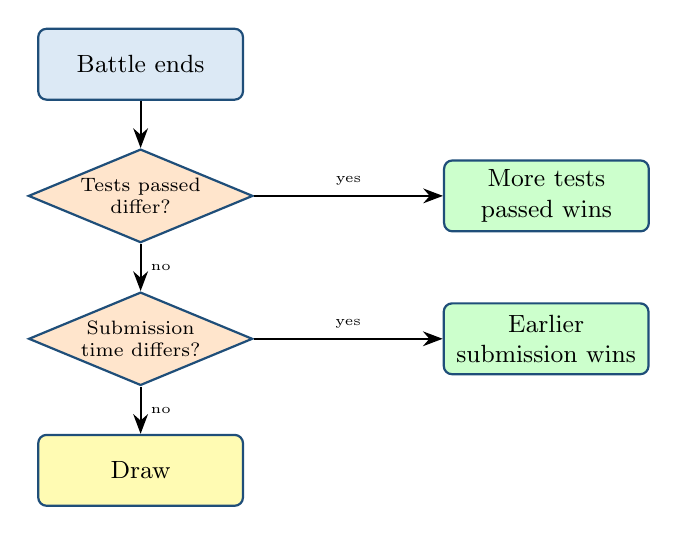
\begin{tikzpicture}[node distance=0.6cm,
  dec/.style={diamond,draw=cdblue,fill=orange!20,thick,aspect=2.4,font=\scriptsize,align=center,inner sep=1pt}]
  \node[box] (a) {Battle ends};
  \node[dec,below=of a] (b) {Tests passed\\differ?};
  \node[box,right=2.4cm of b,fill=green!20] (w1) {More tests\\passed wins};
  \node[dec,below=of b] (c) {Submission\\time differs?};
  \node[box,right=2.4cm of c,fill=green!20] (w2) {Earlier\\submission wins};
  \node[box,below=of c,fill=yellow!30] (d) {Draw};
  \draw[arr] (a)--(b);
  \draw[arr] (b)--(w1) node[midway,above,font=\tiny]{yes};
  \draw[arr] (b)--(c) node[midway,right,font=\tiny]{no};
  \draw[arr] (c)--(w2) node[midway,above,font=\tiny]{yes};
  \draw[arr] (c)--(d) node[midway,right,font=\tiny]{no};
\end{tikzpicture}
\caption{Winner determination flow}
\end{figure}

\section{Elo Rating System}
Let $R_A$ and $R_B$ be the ratings of players A and B. The expected score of A is
\[
  E_A = \frac{1}{1 + 10^{(R_B - R_A)/400}},
\]
and the updated rating is
\[
  R_A' = R_A + K\,(S_A - E_A),
\]
where $S_A \in \{1, 0.5, 0\}$ for a win, draw or loss and $K$ is the development constant (here $K = 32$).

\textbf{Worked example.} Aryan (1250) defeats Rahul (1280): $E_A = 1/(1+10^{30/400}) \approx 0.457$.
Then $R_A' = 1250 + 32(1 - 0.457) \approx 1267$ and $R_B' = 1280 + 32(0 - 0.543) \approx 1263$.

\begin{figure}[H]
\centering
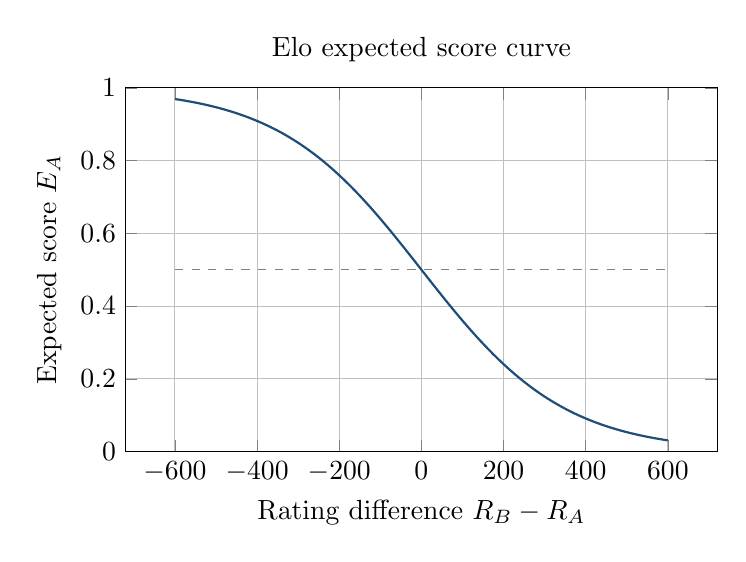
\begin{tikzpicture}
\begin{axis}[width=0.75\textwidth,height=6.2cm,xlabel={Rating difference $R_B - R_A$},
  ylabel={Expected score $E_A$},grid=major,domain=-600:600,samples=100,
  ymin=0,ymax=1,title={Elo expected score curve}]
  \addplot[thick,cdblue] {1/(1+10^(x/400))};
  \addplot[dashed,gray] coordinates {(-600,0.5)(600,0.5)};
\end{axis}
\end{tikzpicture}
\caption{Expected score of player A as a function of rating difference}
\end{figure}

\section{Frontend Implementation}
The React application is divided into pages (Login, Home, Matchmaking, Battle, Results, Profile,
Leaderboard) and reusable components (CodeEditor, ProblemPanel, Timer, PlayerCard, SubmissionResult).
The Monaco editor is embedded through a wrapper component; a \texttt{websocket.js} service manages the STOMP
connection, subscribes to \texttt{/topic/battle/\{id\}} and dispatches events to the UI state. An
\texttt{AuthContext} stores the JWT and the current user.

\begin{lstlisting}[language=Java,caption={Client-side STOMP subscription (JavaScript)},numbers=none]
// services/websocket.js
const client = new Client({ brokerURL: WS_URL,
  connectHeaders: { Authorization: `Bearer ${token}` } });
client.onConnect = () => {
  client.subscribe(`/topic/battle/${battleId}`, msg => {
    const event = JSON.parse(msg.body);
    dispatch(event);   // PLAYER_JOINED, BATTLE_STARTED, ...
  });
};
client.activate();
\end{lstlisting}

\section{Deployment}
The entire system is containerised and started with Docker Compose.
\begin{figure}[H]
\centering
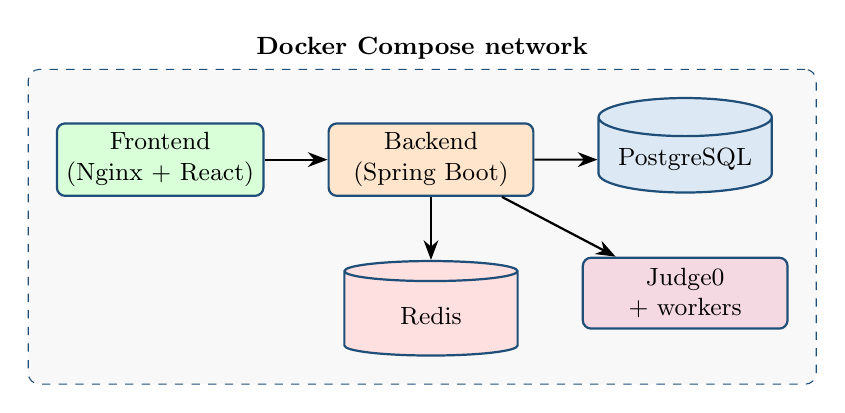
\begin{tikzpicture}[node distance=0.8cm]
  \node[box,fill=green!15] (fe) {Frontend\\(Nginx + React)};
  \node[box,right=of fe,fill=orange!20] (be) {Backend\\(Spring Boot)};
  \node[dbox,right=of be] (db) {PostgreSQL};
  \node[dbox,below=of be,fill=red!12] (rd) {Redis};
  \node[box,below=of db,fill=purple!15] (j0) {Judge0\\+ workers};
  \draw[arr] (fe)--(be); \draw[arr] (be)--(db); \draw[arr] (be)--(rd); \draw[arr] (be)--(j0);
  \begin{scope}[on background layer]
    \node[draw=cdblue,dashed,rounded corners,fit=(fe)(be)(db)(rd)(j0),inner sep=0.35cm,fill=cdgrey!50,
          label={[font=\small\bfseries]above:Docker Compose network}] {};
  \end{scope}
\end{tikzpicture}
\caption{Deployment view using Docker Compose}
\end{figure}

% ---------------------------------------------------------------------
\chapter{Security Considerations}
% ---------------------------------------------------------------------
\begin{table}[H]
\centering
\small
\begin{tabularx}{\textwidth}{@{}lX@{}}
\toprule
\textbf{Threat} & \textbf{Countermeasure} \\
\midrule
Malicious code (fork bombs, file access) & Executed only inside Judge0/Docker with CPU, memory, process and time limits; network disabled. \\
Stolen credentials & BCrypt password hashing; short-lived JWT; HTTPS in production. \\
Client tampering with result/timer & Client never decides winner; server owns timer and verdict. \\
Hidden-test leakage & Hidden test cases never sent to client; only pass counts returned. \\
Opponent code exposure & Only status and pass count broadcast over WebSocket. \\
Submission spam / DoS & Rate limiting per user; repeated identical submissions detected. \\
Unauthorised battle access & WebSocket handshake authenticated; user must be a participant of the battle. \\
SQL injection & Parameterised queries via Spring Data JPA. \\
\bottomrule
\end{tabularx}
\caption{Threats and mitigations}
\end{table}

\begin{quote}
\textbf{Principle:} \emph{The client is untrusted. All decisions about correctness, time and winner are made on the server.}
\end{quote}

% ---------------------------------------------------------------------
\chapter{Testing}
% ---------------------------------------------------------------------
\section{Testing Strategy}
\begin{itemize}[leftmargin=*]
  \item \textbf{Unit testing:} JUnit/Mockito for services (rating, winner logic, matchmaking).
  \item \textbf{Integration testing:} Spring Boot Test with a test PostgreSQL/Redis container.
  \item \textbf{API testing:} Postman collections for all REST endpoints.
  \item \textbf{WebSocket testing:} Two simultaneous browser sessions and scripted STOMP clients.
  \item \textbf{Security testing:} Invalid tokens, tampered payloads, infinite-loop and memory-bomb submissions.
\end{itemize}

\section{Sample Test Cases}
\begin{table}[H]
\centering
\small
\begin{tabularx}{\textwidth}{@{}llXl@{}}
\toprule
\textbf{ID} & \textbf{Module} & \textbf{Test description / expected result} & \textbf{Status} \\
\midrule
TC01 & Auth & Register with valid data creates a user & Pass \\
TC02 & Auth & Login with wrong password returns 401 & Pass \\
TC03 & Auth & Request without JWT is rejected & Pass \\
TC04 & Matchmaking & Two players within range are matched & Pass \\
TC05 & Matchmaking & Window widens after 10 s and matches distant players & Pass \\
TC06 & Battle & Both players receive BATTLE\_STARTED together & Pass \\
TC07 & Judge & Correct solution returns ACCEPTED with all tests passed & Pass \\
TC08 & Judge & Infinite loop terminates with TIME\_LIMIT & Pass \\
TC09 & Judge & Syntax error returns COMPILATION\_ERROR & Pass \\
TC10 & Winner & More tests passed beats earlier submission & Pass \\
TC11 & Rating & Winner's rating increases, loser's decreases & Pass \\
TC12 & Security & Opponent source code is not present in any WS message & Pass \\
\bottomrule
\end{tabularx}
\caption{Sample test cases}
\end{table}

% ---------------------------------------------------------------------
\chapter{Results and Analysis}
% ---------------------------------------------------------------------
\begin{center}
\fbox{\parbox{0.92\textwidth}{\small\textbf{Note:} The numerical values in the charts of this chapter are
\emph{illustrative sample data}. Replace them with the measurements you actually obtain from your own
testing before submission.}}
\end{center}

\section{Effort Distribution (Pie Chart)}
\begin{figure}[H]
\centering
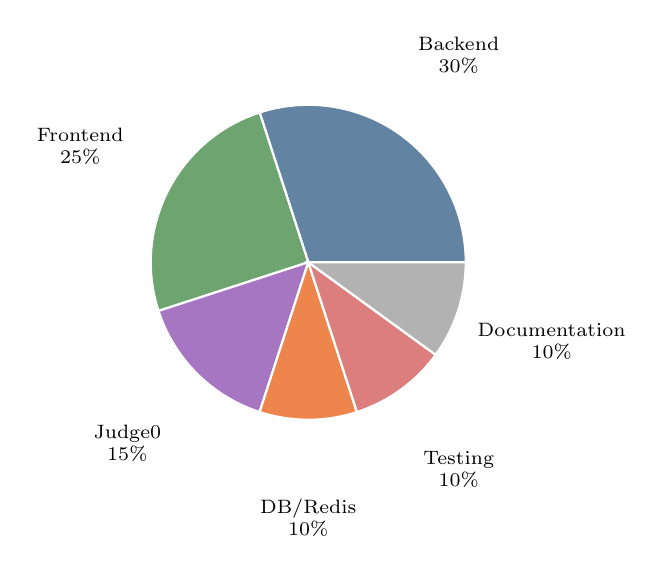
\begin{tikzpicture}
  \pieslice{0}{108}{Backend\\30\%}{cdblue!70}
  \pieslice{108}{198}{Frontend\\25\%}{cdgreen!70}
  \pieslice{198}{252}{Judge0\\15\%}{cdpurple!60}
  \pieslice{252}{288}{DB/Redis\\10\%}{cdorange!70}
  \pieslice{288}{324}{Testing\\10\%}{cdred!60}
  \pieslice{324}{360}{Documentation\\10\%}{gray!60}
\end{tikzpicture}
\caption{Distribution of development effort across project activities}
\end{figure}

\section{Language Usage in Battles (Pie Chart)}
\begin{figure}[H]
\centering
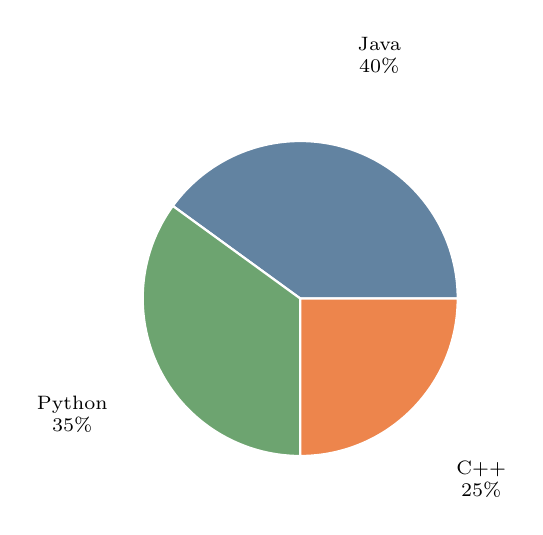
\begin{tikzpicture}
  \pieslice{0}{144}{Java\\40\%}{cdblue!70}
  \pieslice{144}{270}{Python\\35\%}{cdgreen!70}
  \pieslice{270}{360}{C++\\25\%}{cdorange!70}
\end{tikzpicture}
\caption{Share of programming languages used in test battles}
\end{figure}

\section{Judging Time per Language (Bar Chart)}
\begin{figure}[H]
\centering
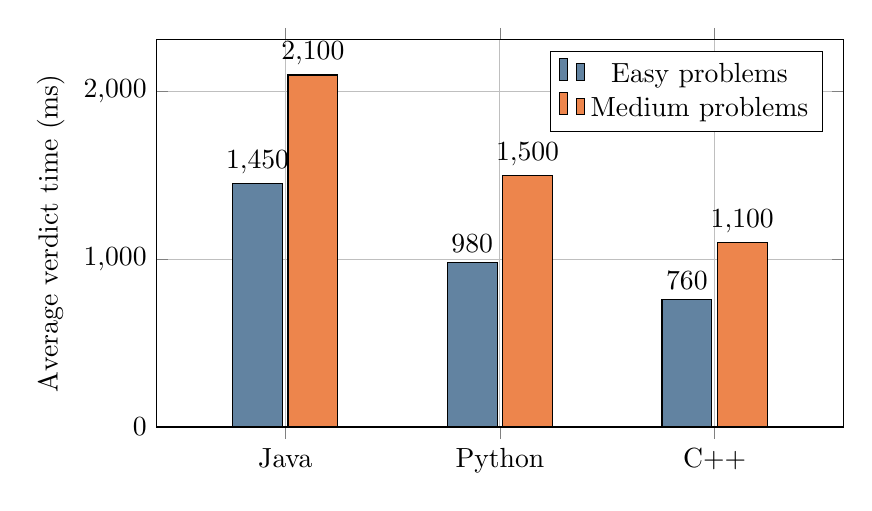
\begin{tikzpicture}
\begin{axis}[ybar,width=0.85\textwidth,height=6.5cm,ylabel={Average verdict time (ms)},
  symbolic x coords={Java,Python,C++},xtick=data,ymin=0,nodes near coords,
  enlarge x limits=0.3,legend pos=north east,
  bar width=18pt,grid=major]
  \addplot[fill=cdblue!70] coordinates {(Java,1450)(Python,980)(C++,760)};
  \addplot[fill=cdorange!70] coordinates {(Java,2100)(Python,1500)(C++,1100)};
  \legend{Easy problems,Medium problems}
\end{axis}
\end{tikzpicture}
\caption{Average judging time by language and difficulty}
\end{figure}

\section{Matchmaking Wait Time (Line Chart)}
\begin{figure}[H]
\centering
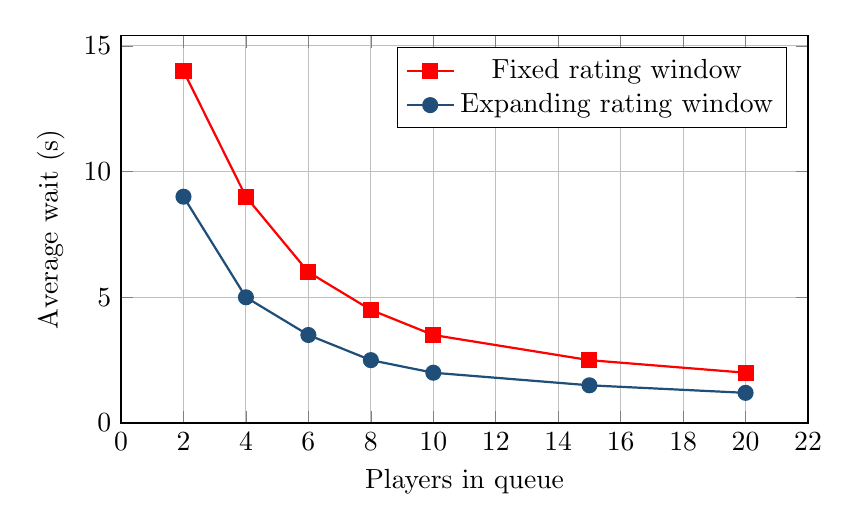
\begin{tikzpicture}
\begin{axis}[width=0.85\textwidth,height=6.5cm,xlabel={Players in queue},ylabel={Average wait (s)},
  grid=major,legend pos=north east,xmin=0,ymin=0,mark size=2.5pt]
  \addplot[thick,red,mark=square*] coordinates {(2,14)(4,9)(6,6)(8,4.5)(10,3.5)(15,2.5)(20,2)};
  \addplot[thick,cdblue,mark=*] coordinates {(2,9)(4,5)(6,3.5)(8,2.5)(10,2)(15,1.5)(20,1.2)};
  \legend{Fixed rating window,Expanding rating window}
\end{axis}
\end{tikzpicture}
\caption{Effect of expanding window on matchmaking wait time}
\end{figure}

\section{Real-Time Event Latency (Bar Chart)}
\begin{figure}[H]
\centering
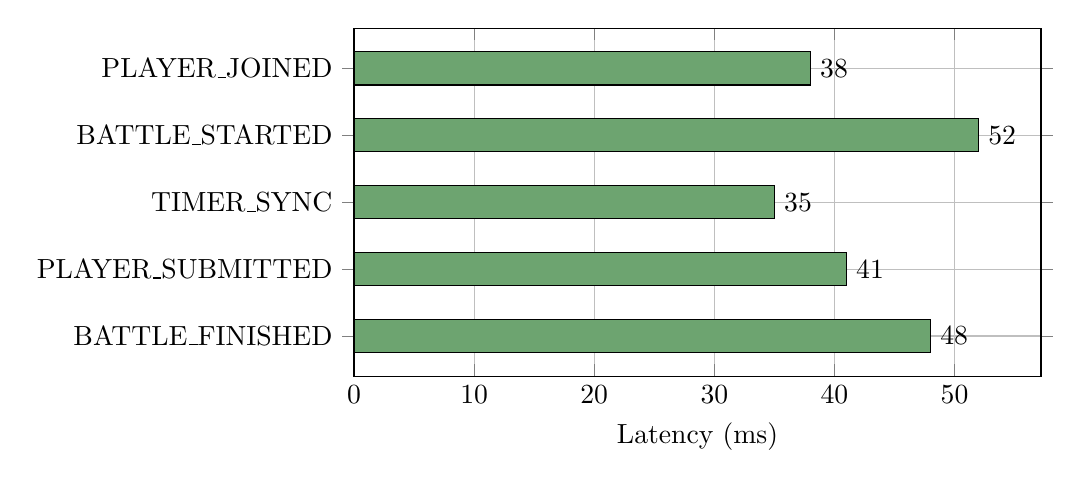
\begin{tikzpicture}
\begin{axis}[xbar,width=0.85\textwidth,height=6cm,xlabel={Latency (ms)},
  symbolic y coords={BATTLE\_FINISHED,PLAYER\_SUBMITTED,TIMER\_SYNC,BATTLE\_STARTED,PLAYER\_JOINED},
  ytick=data,xmin=0,nodes near coords,bar width=12pt,grid=major,enlarge y limits=0.15]
  \addplot[fill=cdgreen!70] coordinates {(48,BATTLE\_FINISHED)(41,PLAYER\_SUBMITTED)(35,TIMER\_SYNC)(52,BATTLE\_STARTED)(38,PLAYER\_JOINED)};
\end{axis}
\end{tikzpicture}
\caption{Average WebSocket event delivery latency}
\end{figure}

\section{Test Results Summary}
\begin{table}[H]
\centering
\small
\begin{tabular}{@{}lccc@{}}
\toprule
\textbf{Module} & \textbf{Tests} & \textbf{Passed} & \textbf{Pass rate} \\
\midrule
Authentication & 12 & 12 & 100\% \\
Matchmaking    & 10 & 10 & 100\% \\
Battle / WebSocket & 14 & 13 & 93\% \\
Judging        & 16 & 16 & 100\% \\
Rating / Winner& 10 & 10 & 100\% \\
Security       & 12 & 12 & 100\% \\
\midrule
\textbf{Total} & \textbf{74} & \textbf{73} & \textbf{99\%} \\
\bottomrule
\end{tabular}
\caption{Summary of testing results (sample data)}
\end{table}

\section{Discussion}
The results show that server-pushed WebSocket events keep both players synchronised with very low latency,
and that the expanding rating window substantially reduces waiting time when the player pool is small
without sacrificing match quality for large pools. Running code in Judge0 adds latency, but this is an
acceptable trade-off for safe execution.

\section{Limitations}
\begin{itemize}[leftmargin=*]
  \item Judging throughput is bounded by the number of Judge0 workers.
  \item The problem set must be curated manually.
  \item Anti-cheating is basic; external assistance cannot be fully prevented.
  \item Elo ratings are less reliable for players with few matches.
\end{itemize}

% ---------------------------------------------------------------------
\chapter{Conclusion and Future Scope}
% ---------------------------------------------------------------------
\section{Conclusion}
CodeDuel demonstrates that a real-time, competitive programming experience can be built with widely
available open-source technologies. The project integrates a reactive front end, a layered Spring Boot
back end, real-time WebSocket communication, Redis-backed matchmaking, secure sandboxed execution and a
rating system into a cohesive product. The design principle of never trusting the client, together with
container isolation, provides a secure basis for running untrusted code. The phased approach shows how a
complex distributed application can be delivered incrementally.

\section{Future Scope}
\begin{itemize}[leftmargin=*]
  \item Tournament and league modes; daily challenges; achievements.
  \item Spectator mode and battle replay from stored events.
  \item Advanced anti-cheat: plagiarism similarity detection and tab-switch monitoring.
  \item Team battles and friend system.
  \item Horizontal scaling with Redis Pub/Sub and Kubernetes.
  \item AI-based hint and post-battle feedback system.
\end{itemize}

% ---------------------------------------------------------------------
%  Appendix: project schedule
% ---------------------------------------------------------------------
\appendix
\chapter{Project Schedule (Gantt Chart)}
\begin{figure}[H]
\centering
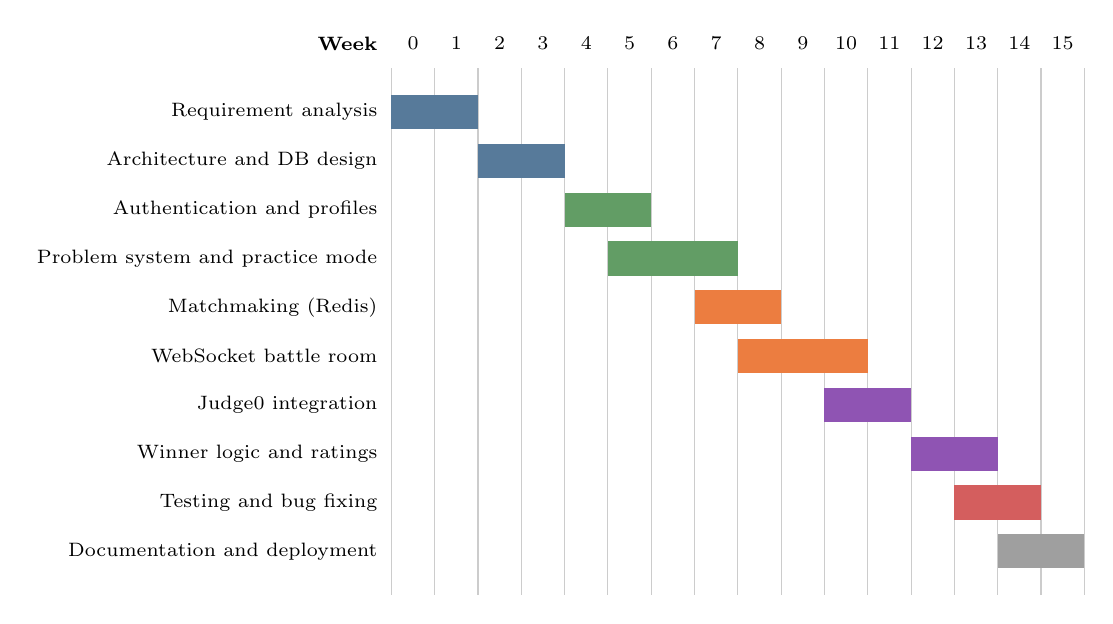
\begin{tikzpicture}[x=0.55cm,y=-0.62cm,font=\scriptsize]
  % week grid
  \foreach \w in {0,...,16} {
    \draw[gray!40] (\w,-0.4) -- (\w,10.4);
    \ifnum\w<16 \node at (\w+0.5,-0.9) {\w}; \fi
  }
  \node[anchor=east] at (-0.1,-0.9) {\textbf{Week}};
  \def\tasks{
    1/Requirement analysis/0/2/cdblue,
    2/Architecture and DB design/2/4/cdblue,
    3/Authentication and profiles/4/6/cdgreen,
    4/Problem system and practice mode/5/8/cdgreen,
    5/Matchmaking (Redis)/7/9/cdorange,
    6/WebSocket battle room/8/11/cdorange,
    7/Judge0 integration/10/12/cdpurple,
    8/Winner logic and ratings/12/14/cdpurple,
    9/Testing and bug fixing/13/15/cdred,
    10/Documentation and deployment/14/16/gray}
  \foreach \i/\n/\s/\e/\c in \tasks {
    \node[anchor=east] at (-0.1,\i-0.5) {\n};
    \fill[\c!75] (\s,\i-0.85) rectangle (\e,\i-0.15);
  }
\end{tikzpicture}
\caption{Project timeline (16 weeks)}
\end{figure}

\chapter{Sample Problem Definition}
\begin{lstlisting}[language=,numbers=none,caption={Example problem record: Two Sum}]
title:        Two Sum
difficulty:   Easy
description:  Given an array of integers nums and an integer target,
              return indices of the two numbers that add up to target.
constraints:  2 <= nums.length <= 10^4
visible tests: 3      hidden tests: 10
time limit:   2 s     memory limit: 256 MB
example:      nums = [2,7,11,15], target = 9  ->  [0,1]
\end{lstlisting}

% ---------------------------------------------------------------------
%  References
% ---------------------------------------------------------------------
\begin{thebibliography}{99}
\addcontentsline{toc}{chapter}{References}
\bibitem{spring} Spring Framework Documentation -- WebSocket and STOMP Messaging, \url{https://docs.spring.io/spring-framework/reference/web/websocket.html}.
\bibitem{boot} Spring Boot Reference Documentation, \url{https://docs.spring.io/spring-boot/}.
\bibitem{secu} Spring Security Reference, \url{https://docs.spring.io/spring-security/reference/}.
\bibitem{react} React Documentation, \url{https://react.dev}.
\bibitem{monaco} Monaco Editor, Microsoft, \url{https://microsoft.github.io/monaco-editor/}.
\bibitem{judge0} Judge0 -- Open Source Online Code Execution System, \url{https://judge0.com}.
\bibitem{redis} Redis Documentation, \url{https://redis.io/docs/}.
\bibitem{pg} PostgreSQL Documentation, \url{https://www.postgresql.org/docs/}.
\bibitem{docker} Docker Documentation, \url{https://docs.docker.com}.
\bibitem{elo} A.~E.~Elo, \emph{The Rating of Chessplayers, Past and Present}, Arco Publishing, 1978.
\bibitem{jwt} M.~Jones, J.~Bradley, N.~Sakimura, ``JSON Web Token (JWT),'' RFC 7519, IETF, 2015.
\bibitem{ws} I.~Fette and A.~Melnikov, ``The WebSocket Protocol,'' RFC 6455, IETF, 2011.
\end{thebibliography}

\end{document}